\subsubsection{Caso d'uso UC8.2.7: Modifica domanda con area cliccabile nell'immagine}
\label{UC8.2.7}
\begin{figure}[h]
	\centering
	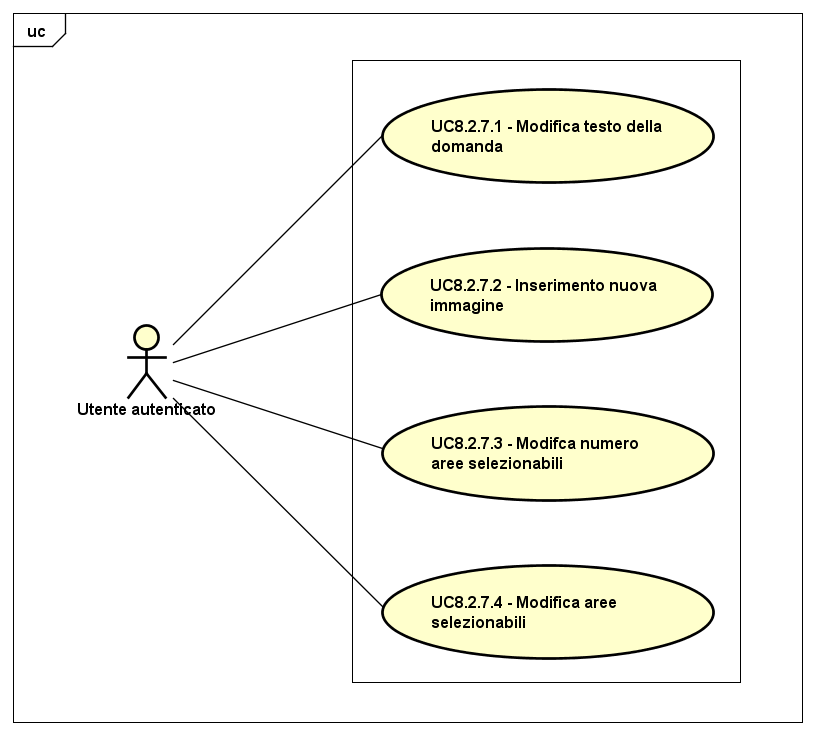
\includegraphics[scale=0.5,keepaspectratio]{UML/UC8_2_7.png}
	\caption{UC8.2.7: Modifica domanda con area cliccabile nell'immagine}
\end{figure}
\FloatBarrier
\begin{itemize}
	\item \textbf{Attori}: utente autenticato, utente autenticato pro;
	\item \textbf{Descrizione}: l'attore può utilizzare la procedura guidata per la modifica di una domanda la cui risposta è selezionabile all'interno di aree cliccabili in un'immagine;
	\item \textbf{Precondizione}:  il sistema ha ricevuto dall'attore la domanda da modificare; 
	\item \textbf{Postcondizione}: l'attore ha modificato una domanda con area cliccabile nell'immagine;
	\item \textbf{Scenario principale}:
		\begin{enumerate}
	       	\item L'attore può modificare il testo della domanda (UC8.2.7.1);
	        \item L'attore può modificare l'immagine relativa al testo della domanda (UC8.2.7.2);
			\item L'attore può scegliere un nuovo numero di aree che saranno selezionabili all'interno dell'immagine (UC8.2.7.3);
			\item L'attore può scegliere nuove aree selezionabili all'interno dell'immagine (UC8.2.7.4);
	 	\end{enumerate}
\end{itemize}

\subsubsection{Caso d'uso UC8.2.7.1: Modifica testo della domanda}
\begin{itemize}
	\item \textbf{Attori}: utente autenticato, utente autenticato pro;
	\item \textbf{Descrizione}: l'attore può modificare il testo della domanda;
	\item \textbf{Precondizione}: il sistema mostra la funzionalità di modifica di una domanda con area cliccabile nell'immagine; 
	\item \textbf{Postcondizione}: l'attore ha modificato il testo della domanda;
	\item \textbf{Scenario principale}: l'attore modifica il testo della domanda. 
\end{itemize}

\subsubsection{Caso d'uso UC8.2.7.2: Inserimento nuova immagine}
\begin{itemize}
	\item \textbf{Attori}: utente autenticato, utente autenticato pro;
	\item \textbf{Descrizione}: l'attore può inserire una nuova immagine relativa al testo della domanda che sostituisce quella già presente;
	\item \textbf{Precondizione}: il sistema mostra la funzionalità di modifica di una domanda con area cliccabile nell'immagine; 
	
	\item \textbf{Postcondizione}: l'attore ha inserito una nuova immagine;
	\item \textbf{Scenario principale}: l'attore inserisce una nuova immagine al posto di quella che era presente. 	
\end{itemize}

\subsubsection{Caso d'uso UC8.2.7.3: Modifica numero aree selezionabili}
\begin{itemize}
	\item \textbf{Attori}: utente autenticato, utente autenticato pro;
	\item \textbf{Descrizione}: l'attore può scegliere un nuovo numero di aree selezionabili all'interno dell'immagine;
	\item \textbf{Precondizione}: il sistema mostra la funzionalità di modifica di una domanda con area cliccabile nell'immagine; 
	
	\item \textbf{Postcondizione}: l'attore ha scelto il nuovo numero di aree selezionabili all'interno dell'immagine;
	\item \textbf{Scenario principale}: l'attore sceglie il nuovo numero di aree selezionabili all'interno dell'immagine. 	
\end{itemize}

\subsubsection{Caso d'uso UC8.2.7.4: Modifica aree selezionabili}
\begin{itemize}
	\item \textbf{Attori}: utente autenticato, utente autenticato pro;
	\item \textbf{Descrizione}: l'attore può scegliere dove inserire le nuove aree selezionabili o riposizionare quelle già presenti all'interno dell'immagine;
	\item \textbf{Precondizione}: il sistema mostra la funzionalità di modifica di una domanda con area cliccabile nell'immagine; 
	
	\item \textbf{Postcondizione}: l'attore ha scelto dove inserire le nuove aree selezionabili o dove riposizionare quelle già presenti all'interno dell'immagine;
	\item \textbf{Scenario principale}: l'attore sceglie dove inserire le nuove aree selezionabili o riposiziona quelle già presenti all'interno dell'immagine. 	
\end{itemize}
